%\DocumentMetadata{pdfversion=2.0,pdfstandard=A-4,tagging=on,lang=zh}
\documentclass[12pt]{article}

%引入宏包
\usepackage{hyperref}
\usepackage{unicode-math}
\usepackage{geometry}
\usepackage{babel}
\usepackage{indentfirst}
\usepackage{fontspec}
\usepackage{luatexja}
\usepackage{luatexja-fontspec}
\usepackage{amsmath}
\usepackage{ragged2e}
\usepackage{float}
\usepackage{booktabs}
\usepackage{graphicx}
\usepackage{multicol}
\usepackage{tikz}
\usepackage[backend=biber,style=gb7714-2015ms]{biblatex}

%Tikz
\usetikzlibrary{intersections,calc,shapes.callouts}

%语言设置
\babelprovide[import,main]{chinese}
\babelprovide[import]{english}

%字体设置
\setmainfont{Times New Roman}[BoldFont=SimHei]
\setmainjfont{NSimSun}[BoldFont=SimHei]
\setsansfont{SimHei}
\setsansjfont{SimHei}

\newjfontfamily{\heiti}{SimHei}
\newjfontfamily{\kaiti}{KaiTi}

%段落格式
\linespread{1.2}
\setlength{\parskip}{8pt}
\setlength{\parindent}{24pt}

%引用设置
\hypersetup{colorlinks,allcolors=blue}

%纸张设置
\geometry{a4paper,margin=1.5cm}

%参考文献
\addbibresource{./bibliography.bib}

%重定义
\renewenvironment{abstract}{
	\begin{center}
		\large \heiti 摘要
	\end{center}

	\vspace{2ex}

}{
}


%文档信息
\title{\heiti 机械工程测试技术报告}
\author{石成玉}
\date{\today}

\begin{document}

\maketitle

\begin{abstract}
	土壤肥力直接影响果树的生长、产量和品质及果园的可持续健康发展。土壤有机质是衡量土壤肥力的重要标准，决定了土壤肥力的物质基础，也是保障果树高产、优质的重要条件。果园施用有机肥可以有效增加土壤有机质含量，改善土壤结构及理化性状，是果园产业实现高质量高效率发展的关键之一。

	目前，果园有机肥施肥机已进行了大量研究，但由于高湿有机肥容易与肥箱底板内部粘附，导致施肥机排肥装置阻力增大，严重时会引起肥料堵塞现象，极大的影响了作业质量与效率，因此减小有机肥施肥机排肥作业阻力已成为亟待解决的问题。

	超声波技术在其他领域已经有很多应用，为了将超声波减黏降阻技术在农业机械中应用，解决有机肥施肥机阻力大、堵塞的问题，本文利用机械工程测试技术对超声波减阻效果和规律进行探究。并将测试技术应用在控制装置中。
\end{abstract}

\section{前言}

中国水果产业品类多、总量大，水果产业已经成为了中国继粮食、蔬菜之后的第三农业种植产业，果园总面积和水果总产量年稳居世界首位。我国果品的生产总量、栽培面积及资源种类均居于世界首位，国家统计局数据显示，2022年，中国水果产量为31296.24万吨，同比增长4.42\%。我国虽然是世界水果生产大国之一，但并不是世界水，果生产强国\parencite{__2022}，我国水果产业没有充分发挥我国所有的自然资源优势。其中，我国水果出口贸易发展中存在的国际影响力弱，水果竞争力弱等问题，最根本的原因是我国果品品质差、劣质品种多。

水果产业的优质发展不仅需要充足的营养，还需要有良好的果园管理技术和方法。果园管理中土壤的养分管理尤其重要，土壤养分条件决定了果品质量以及果园可持续发展(Hoaglandetal.2008)。土壤有机质对果树优质生长发挥了重大的作用(Sunetal.2022；赵丽敏2020)，它富含养分，保证土壤养分供应，支撑水分净化、保持和供应(kayetal.1997)。施用有机肥可以提高微生物群落的生态稳定性、促进果树作物的光合作用，因此施用有机肥对提升果实品质和保护生态环境有着重大意义(王中华2024；刘莉2020)。

果园施肥机械化可以减少生产管理成本，提高施肥作业效率和施肥质量，促进果园肥料高速利用，实现果园增产(刘双喜等2020b)。长久以来我国有机肥施肥方式以人工方式为主，成本较高、劳动强度大(段眉会等2016)。如图\ref{pic:课题组先前研制的有机肥施肥机}所示，课题组先前研究的施肥机施肥过程中易出现肥料与箱底粘附，导致排肥装置工作阻力增大，最终造成有机肥堵塞影响施肥机正常施肥等问题。这是由于有机肥流动性差和含有一定水分的特性导致的，有机肥如图\ref{pic:有机肥}所示。由于农业机械与作物、肥料与土壤等接触作业产生的阻力消耗了大量的动力和能源，因此减阻始终是农业机械设计领域的首要目标(贾洪雷等2017)。

\begin{minipage}{0.45\textwidth}
	\begin{figure}[H]
		\centering

		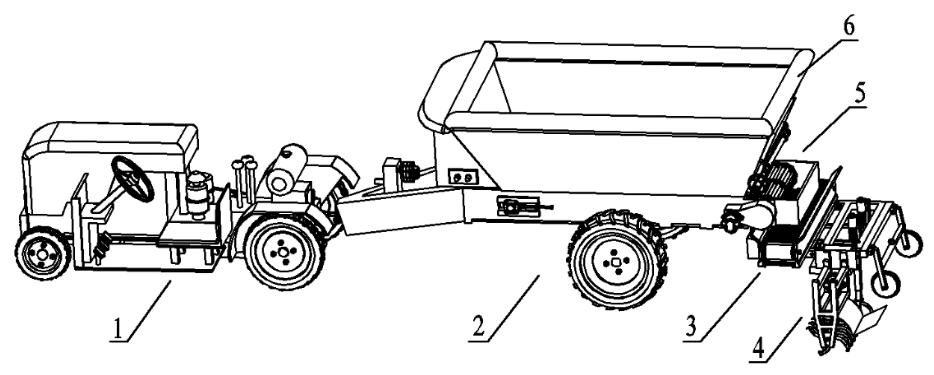
\includegraphics[width=0.4\textwidth]{../../assets/课题组先前研制的有机肥施肥机.png}

		{\kaiti\small 1-拖拉机；2-施肥车；3-抛肥装置；

		4-肥土混合部件；5-排肥装置；6-肥箱；}

		\caption{课题组先前研制的有机肥施肥机}
		\label{pic:课题组先前研制的有机肥施肥机}
	\end{figure}
\end{minipage}
\hfill
\begin{minipage}{0.45\textwidth}
	\begin{figure}[H]
		\centering
		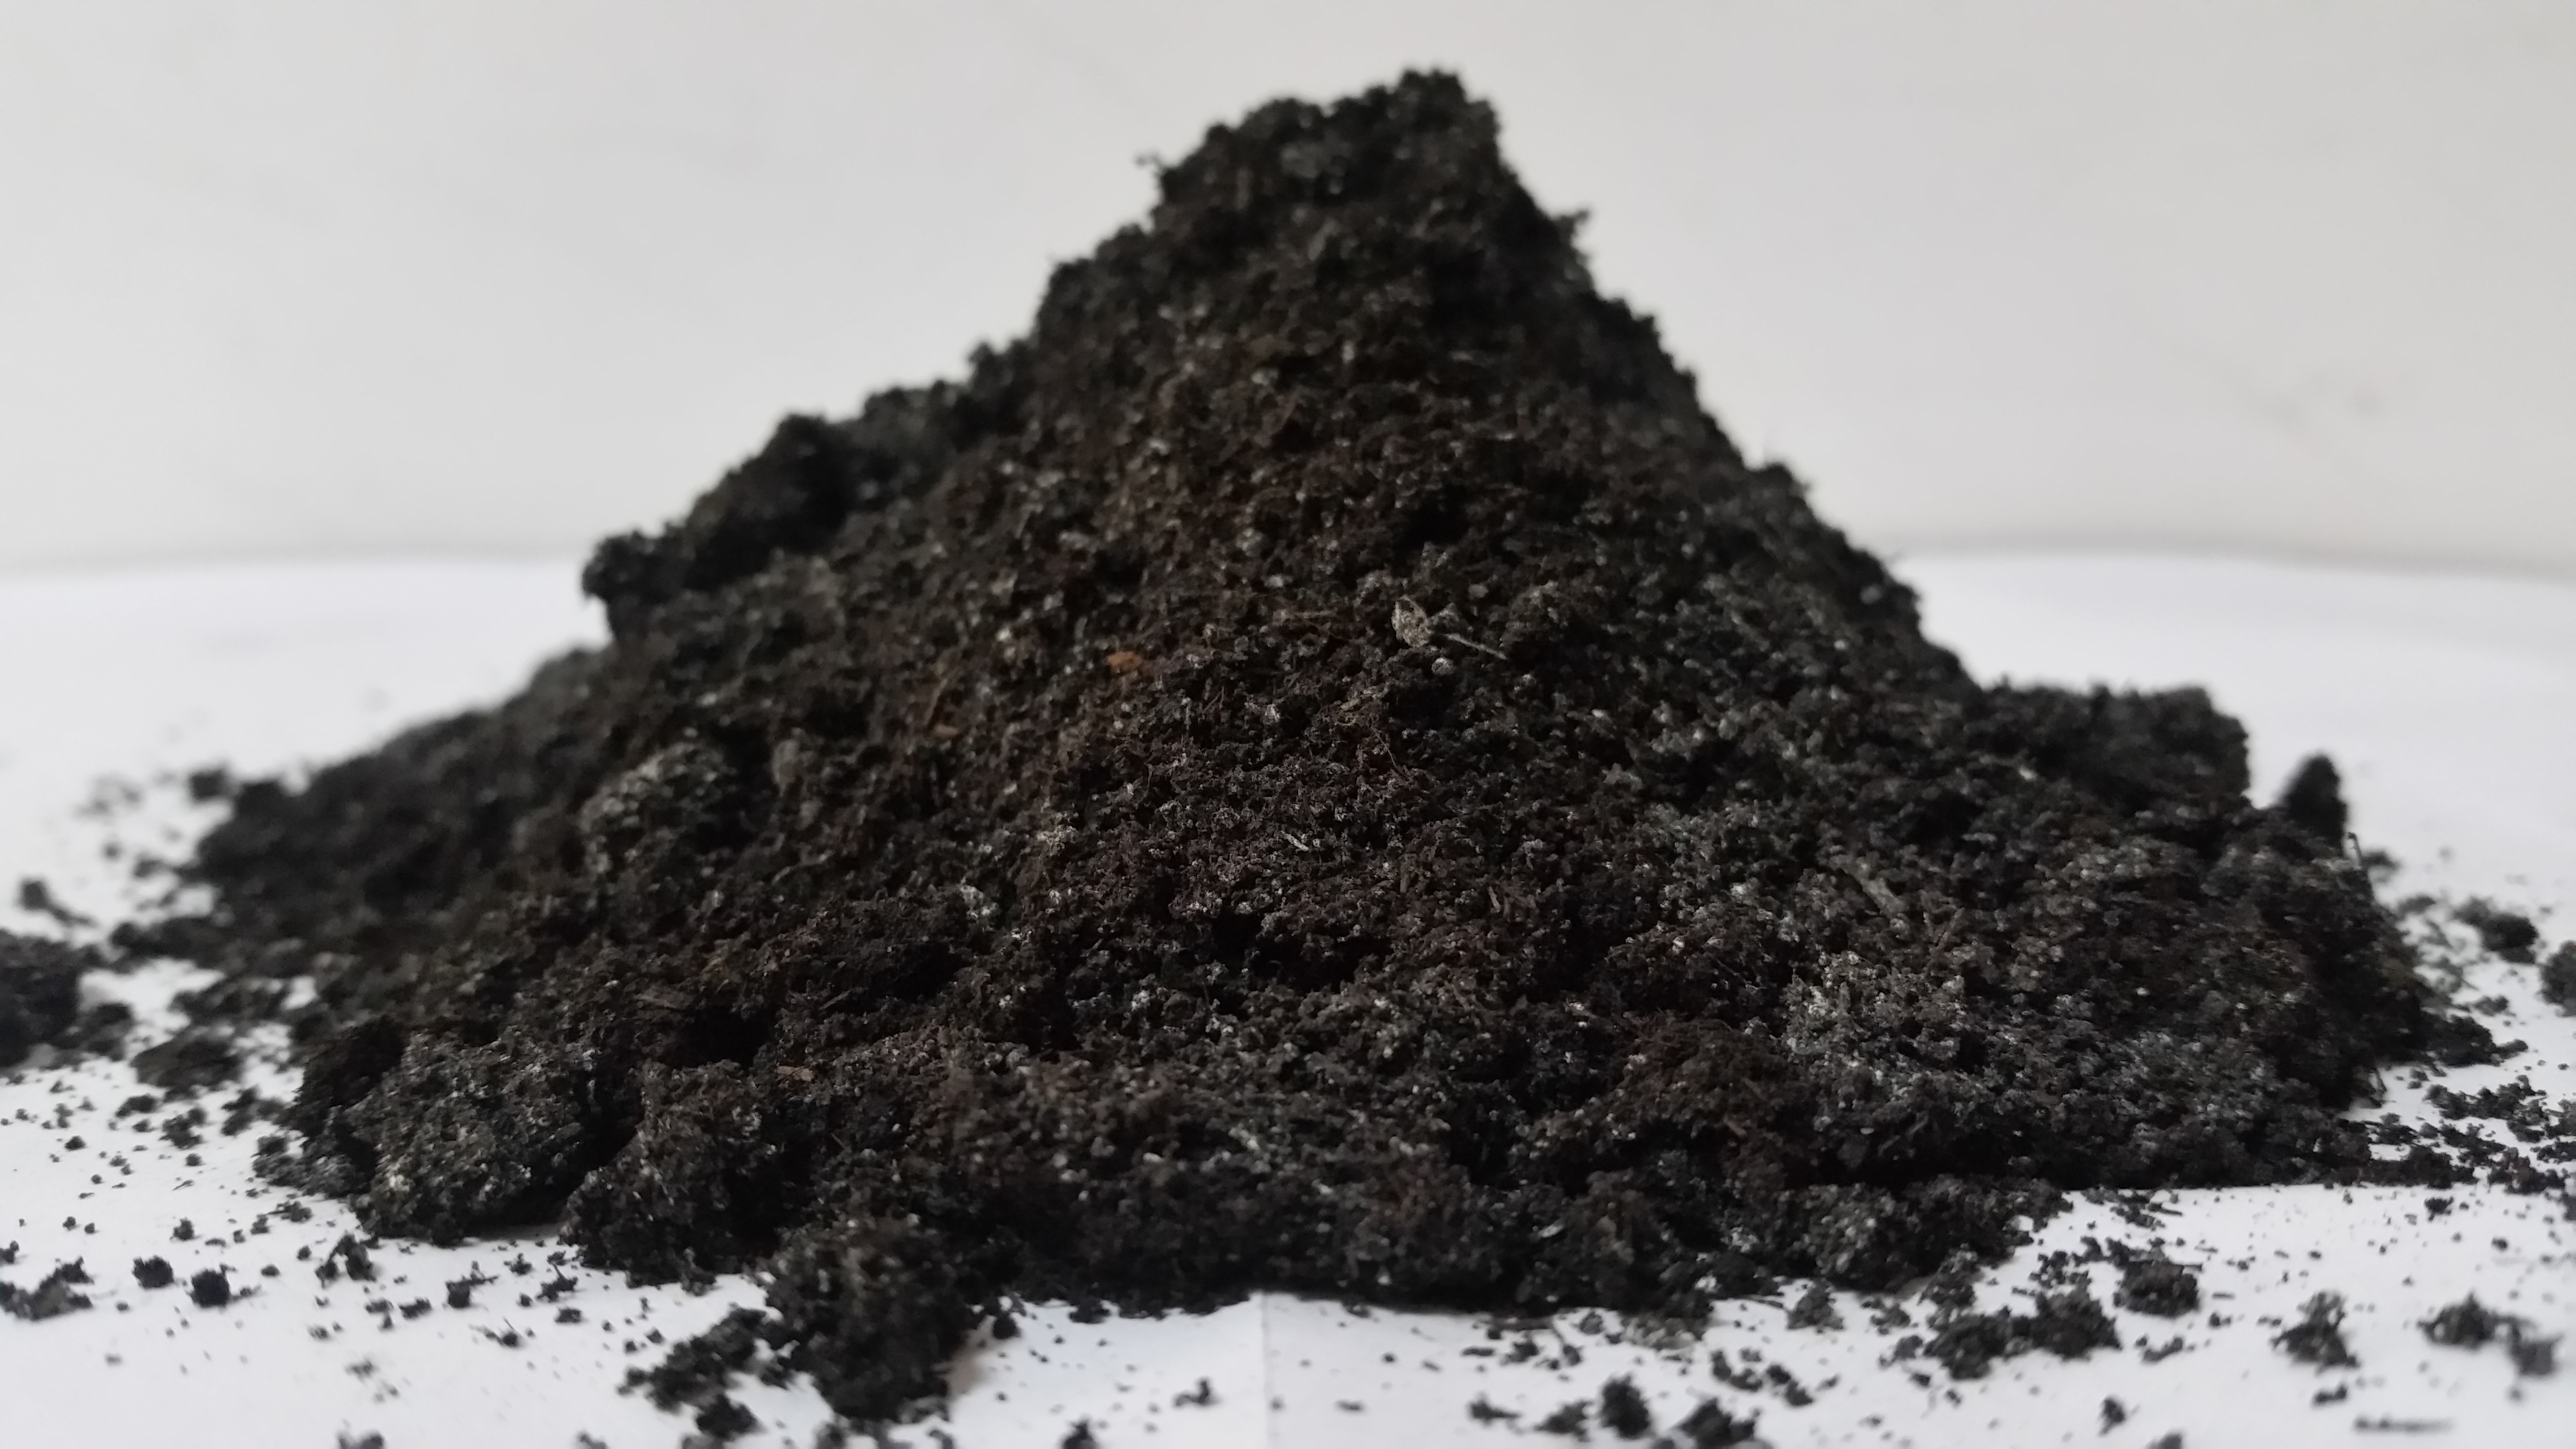
\includegraphics[width=0.4\textwidth]{../../assets/有机肥.png}
		\caption{有机肥}
		\label{pic:有机肥}
	\end{figure}
\end{minipage}

已有研究证明超声振动可在谐振频率范围内降低气缸的摩擦力，提高气缸控制精度(何迪2023)。通过分析，我们可以将超声波振动应用到农业领域。

\section{超声波振动的减阻特性试验}

\subsection{试验方法}

\paragraph{\textbf{斜面仪法}}如图\ref{pic:斜面仪法}所示，将有机肥放置在钢板上，倾斜钢板，记录有机肥开始运动的临界倾角即为摩擦角。再在超声波换能器开启的情况下重复试验，对比即可得到超声波振动对摩擦角的影响效果。

\begin{figure}[H]
	\centering
	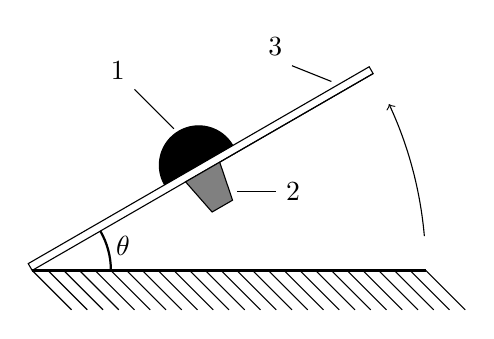
\begin{tikzpicture}
	\begin{scope}[rotate around={30:(0,0)}]
		\draw[fill=white] (0,0) rectangle ($(5,0) + (0,0.1)$);
		\draw[fill=black] ($(2.5,0)+(0.5,0.1)$) arc (0:180:0.5);
		\draw[fill=gray] (5,0) -- ($(2.5,0)+(0.25,0)$) -- ($(2.5,-0.5)+(0.15,0)$) -- ($(2.5,-0.5)-(0.15,0)$) -- ($(2.5,0)-(0.25,0)$) -- cycle;
	\end{scope}
	\draw[thick] (0,0) to (5,0);
	\foreach \x in {0,0.2,...,5}{
		\draw (\x,0) -- ({\x+0.5},-0.5);
	}
	\draw[thick] ($(0,0)+(1,0)$) arc (0:30:1);
	\coordinate (A) at (15:1.2);
	\node[anchor=center] at (A) {$\theta$};
	\coordinate (B) at (1.8,1.8);
	\draw (B) -- +(-0.5,0.5) node[above left]{1};
%	\draw[color=gray,step=0.2] (0,0) grid (5,5);
%	\draw[color=red,step=1] (0,0) grid (5,5);
	\draw (2.6,1) -- +(0.5,0) node[right]{2};
	\draw (3.8,2.4) -- +(-0.5,0.2) node[above left]{3};
	\draw[->] (5:5) arc (5:25:5);
\end{tikzpicture}


	{\kaiti\small 1-有机肥堆；2-超声波换能器；3-钢板；}
	\caption{斜面仪法}
	\label{pic:斜面仪法}
\end{figure}

为了便于比较，定义超声波振动减摩率如式\eqref{eq:减摩率}所示。

\begin{equation}
	\alpha = \frac{\tan{\theta_0}-\tan{\theta_1}}{\tan{\theta_0}} \label{eq:减摩率}
\end{equation}

式中，$\alpha$为超声波振动减摩率；$\theta_0$为有机肥摩擦角；$\theta_1$为超声波振动感激励下的有机肥摩擦角。

\subsection{用到的传感器}

该试验主要使用了倾斜角传感器，其主要工作部分是加速度计（Accelerometer）。加速度计是一种测量加速度向量的传感器。它一般是MEMS（微机电）结构：质量块+弹簧+电容板。

\begin{figure}[H]
	\centering
	\includegraphics[width=0.5\textwidth]{}
\end{figure}

\printbibliography

\end{document}